\documentclass[12pt,a4paper]{exam}
\usepackage[utf8]{inputenc}
\usepackage[T1]{fontenc}
\usepackage{amsmath}
\usepackage{amsfonts}
%\usepackage{amssymb}
\usepackage{graphicx}
\usepackage{geometry}
\usepackage{enumitem}

\geometry{a4paper, margin=2cm}

\usepackage{cprotect}

\usepackage{xcolor}
\definecolor{maroon}{cmyk}{0, 0.87, 0.68, 0.32}
\definecolor{halfgray}{gray}{0.55}
\definecolor{ipython-frame}{RGB}{207, 207, 207}
\definecolor{ipython-bg}{RGB}{247, 247, 247}
\definecolor{ipython-red}{RGB}{186, 33, 33}
\definecolor{ipython-green}{RGB}{0, 128, 0}
\definecolor{ipython-cyan}{RGB}{64, 128, 128}
\definecolor{ipython-purple}{RGB}{170, 34, 255}

\usepackage{listings}
\lstdefinelanguage{iPython}{
	morekeywords={access,and,del,except,exec,in,is,lambda,not,or,raise},
	morekeywords=[2]{for,print,abs,all,any,basestring,bin,bool,bytearray,callable,chr,classmethod,cmp,compile,complex,delattr,dict,dir,divmod,enumerate,eval,execfile,file,filter,float,format,frozenset,getattr,globals,hasattr,hash,help,hex,id,input,int,isinstance,issubclass,iter,len,list,locals,long,map,max,memoryview,min,next,object,oct,open,ord,pow,property,range,reduce,reload,repr,reversed,round,set,setattr,slice,sorted,staticmethod,str,sum,super,tuple,type,unichr,unicode,vars,xrange,zip,apply,buffer,coerce,intern,elif,else,if,continue,break,while,class,def,return,try,except,import,finally,try,except,from,global,pass, True, False},
	sensitive=true,
	morecomment=[l]\#,%
	morestring=[b]',%
	morestring=[b]",%
	moredelim=**[is][\color{black}]{@@}{@@},
	identifierstyle=\color{black}\footnotesize\ttfamily,
	commentstyle=\color{ipython-cyan}\footnotesize\itshape\ttfamily,
	stringstyle=\color{ipython-red}\footnotesize\ttfamily,
	keepspaces=true,
	showspaces=false,
	showstringspaces=false,
	rulecolor=\color{ipython-frame},
	frame=single,
	frameround={t}{t}{t}{t},
	backgroundcolor=\color{ipython-bg},
	basicstyle=\footnotesize\ttfamily,
	keywordstyle=[2]\color{ipython-green}\bfseries\footnotesize\ttfamily, 
	keywordstyle=\color{ipython-purple}\bfseries\footnotesize\ttfamily
}

\lstdefinelanguage{iOutput} {
	sensitive=true,
	identifierstyle=\color{black}\small\ttfamily,
	stringstyle=\color{ipython-red}\small\ttfamily,
	keepspaces=true,
	showspaces=false,
	showstringspaces=false,
	rulecolor=\color{ipython-frame},
	basicstyle=\small\ttfamily,
}

\lstnewenvironment{ipython}[1][]{\lstset{language=iPython,mathescape=true,escapeinside={*@}{@*}}%
}{%
}

\lstnewenvironment{ioutput}[1][]{\lstset{language=iOutput,mathescape=true,escapeinside={*@}{@*}}%
}{%
}

\title{Financial Market Course 25/26\\ Exam}
\author{Prof. Simone Freschi, Prof. Matteo Sani}
\date{$24^{\mathrm{th}}$ September 2026}

%\printanswers
\noprintanswers
\begin{document}
\maketitle

\begin{center}
\fbox{\fbox{\parbox{5.5in}{
Answer the questions in the provided spaces. If you run out of room for an answer, continue on the page back.}}}
\end{center}

\begin{center}
\vspace{5mm}
\makebox[0.75\textwidth]{Student's name:\enspace\hrulefill}
\end{center}

\section*{Questions}
\vspace{.5cm}
\begin{questions}

\question 
Describe what are the main characteristics of a Repo Contract.
\begin{parts}
	\part In the chart I is described the delivery Basket of the BTP Future September 2026 (IKU6) which is currently trading at 114.20. The bond BTPS 3.65 August 2035 is the cheapest to deliver with a price of 97.03 and a conversion factor of 0.8452. Describe if there is an arbitrage opportunity and what kind of strategy would you implement. (\textit{hint}: check the basis and use the cash and carry strategy)
\end{parts}

\makeemptybox{5cm}
\begin{figure}[htb]
	\centering
	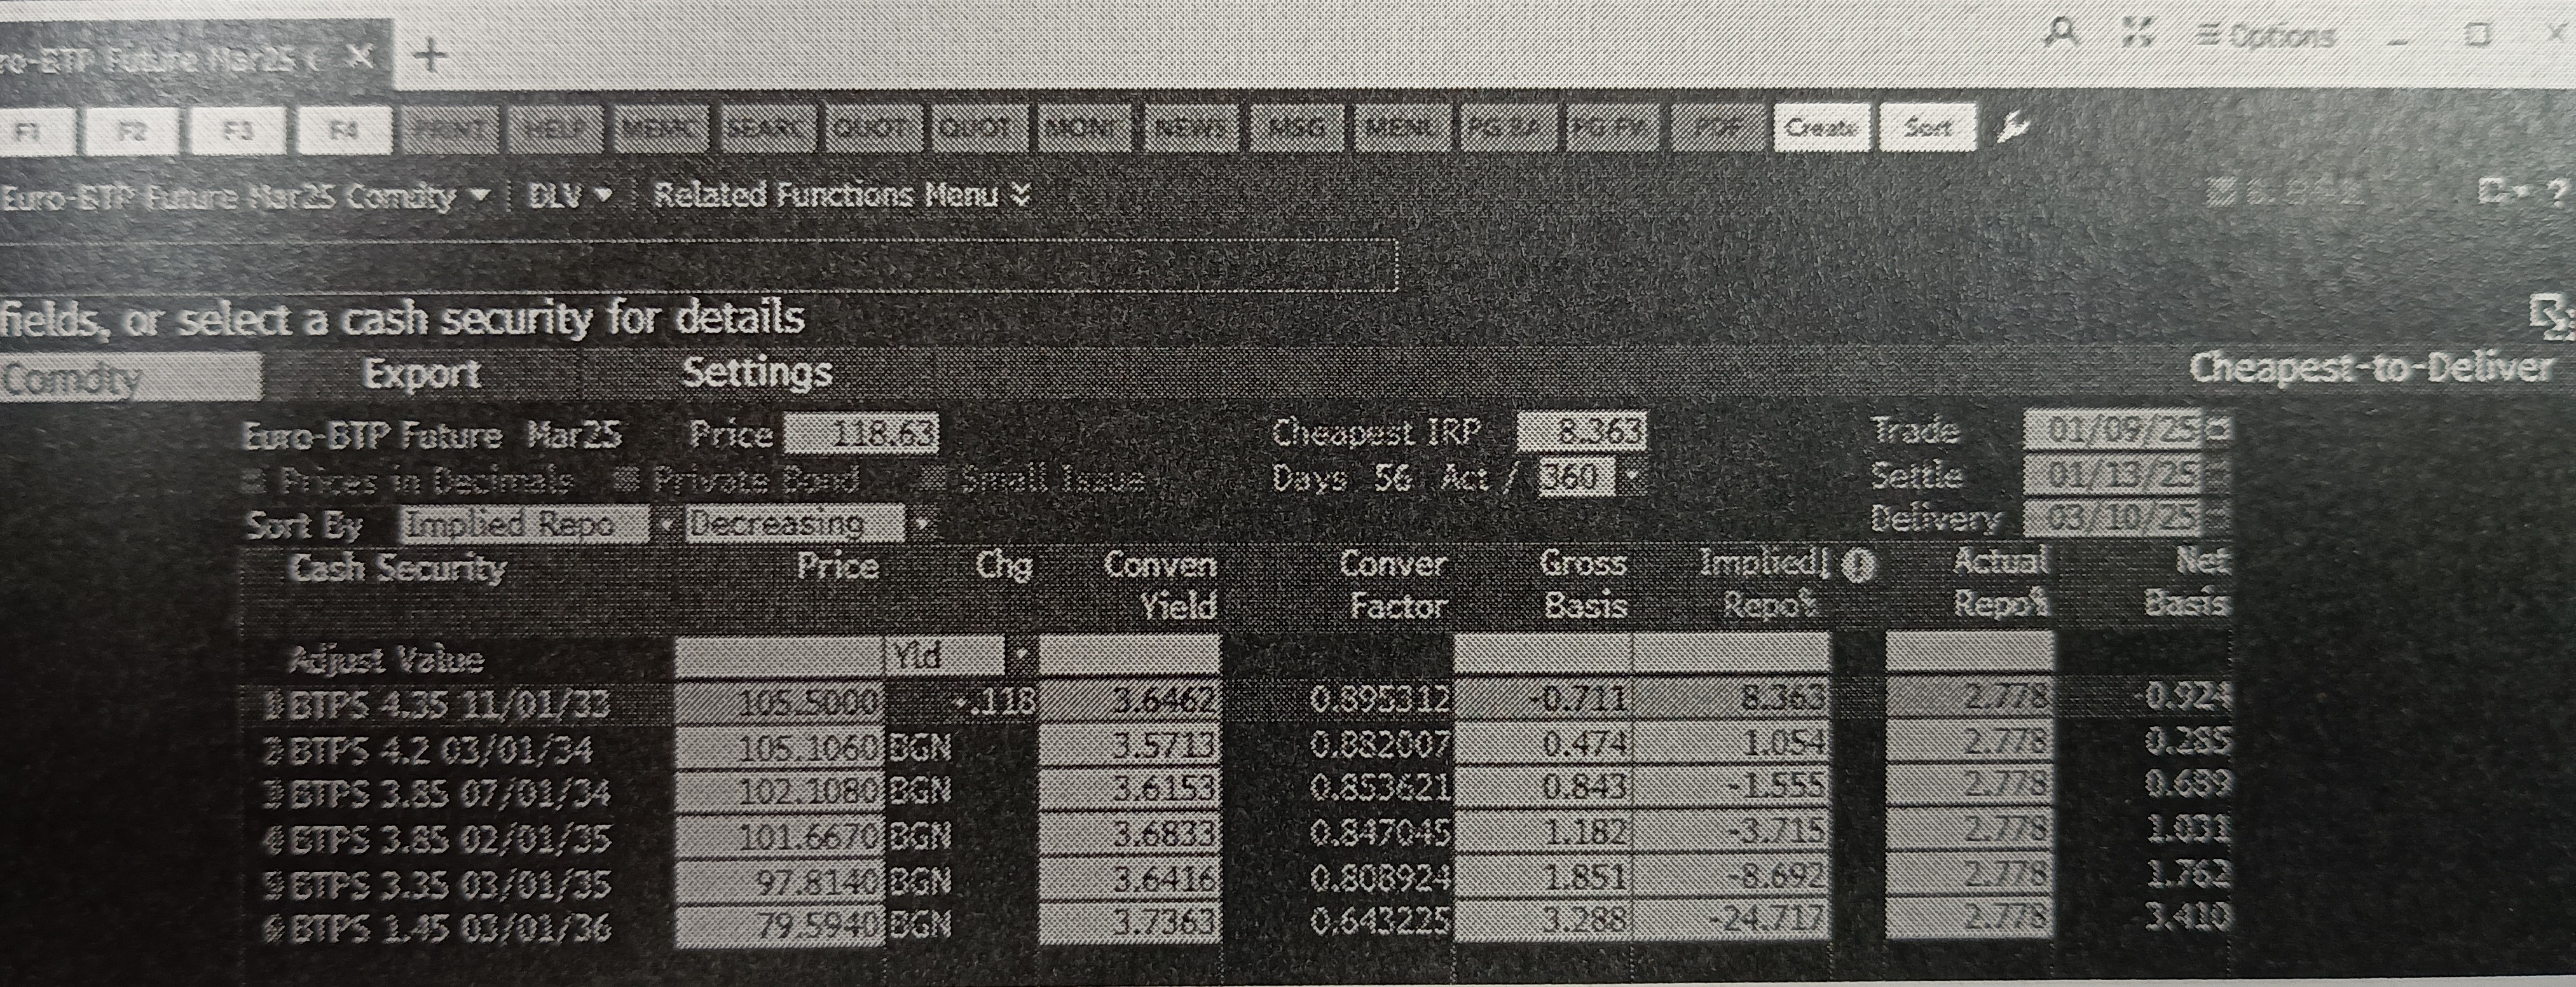
\includegraphics[width=0.9\linewidth]{immagine_compito_27_01_2026}
	\caption{BTP September 2026 Futures}
\end{figure}

\begin{figure}[htb]
	\centering
	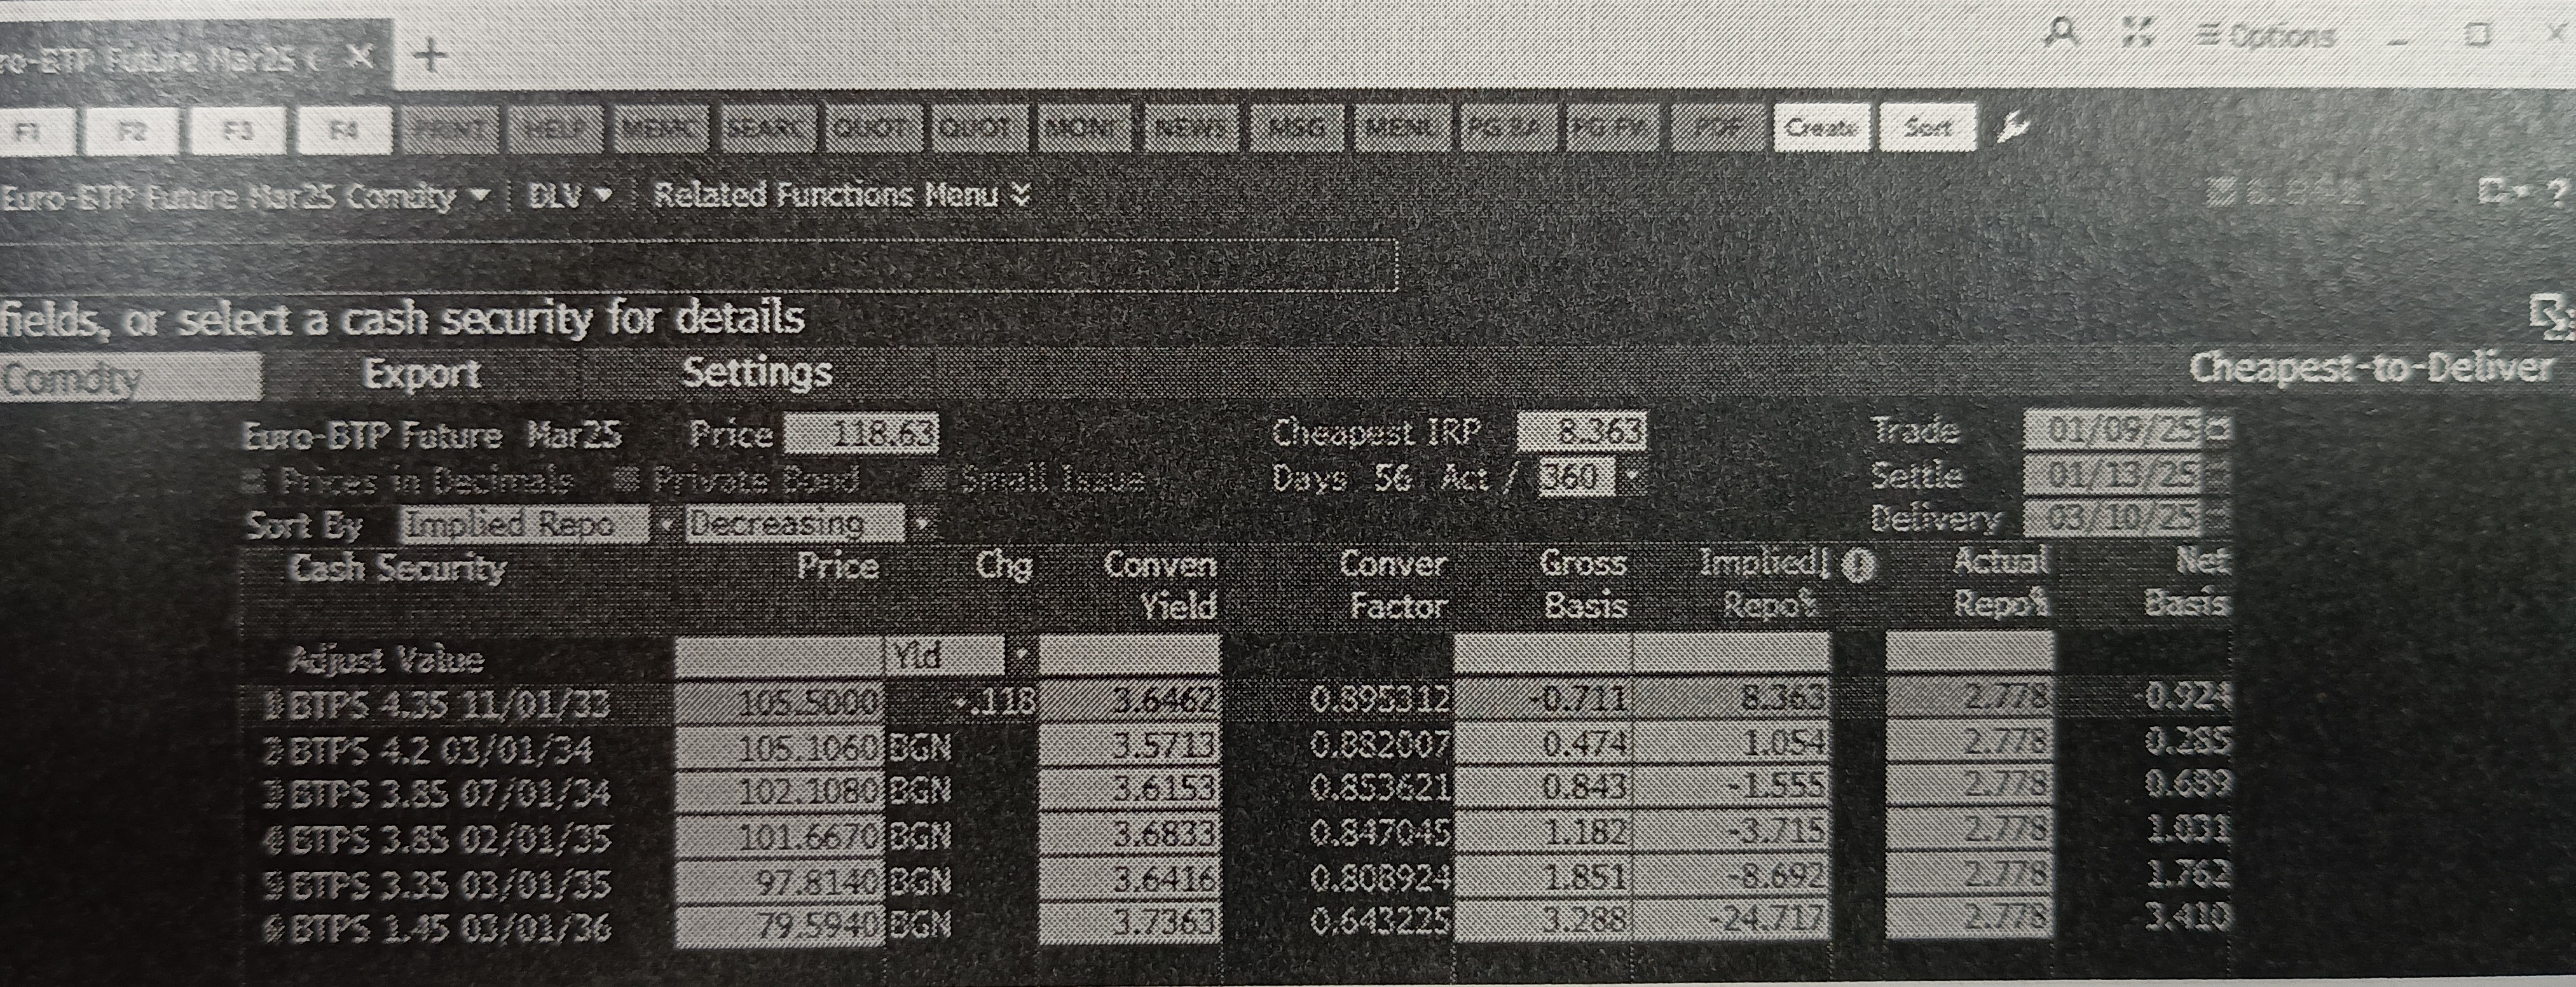
\includegraphics[width=0.9\linewidth]{immagine_compito_27_01_2026}
	\caption{ETF on TIPS}
\end{figure}

%\fillwithdottedlines{5cm}
\begin{solution}
\end{solution}

\question
Inflation Linked Bonds
\begin{parts}
	\part Describe the price in real terms and nominal terms of an Inflation Linked Bond.
	\part Look at the two Bloomberg charts 2 and 3: TIP US (the ETF on US Treasury Inflation Protected with duration of 6.7 years) and USGG10YR Index (US nominal 10Y yield lhs), overlaid with USSWIT10, (thje 10Y inflation swap rate rhs), both Year To Date 2026.
	TIP US has fallen from roughly 112 in late February to below 107 (minus 5\% by September, while the nominal 10Y yield (USGG10YR) has risen from about 4.2\% to nearly 4.8\% over the same period, and the 10Y inflation has moderately increasing (15 bps) since Ytd. According to the previous formula explain if and why the behaviour of the ETF is consisent with ehe market.
\end{parts}

\begin{figure}[htb]
	\centering
	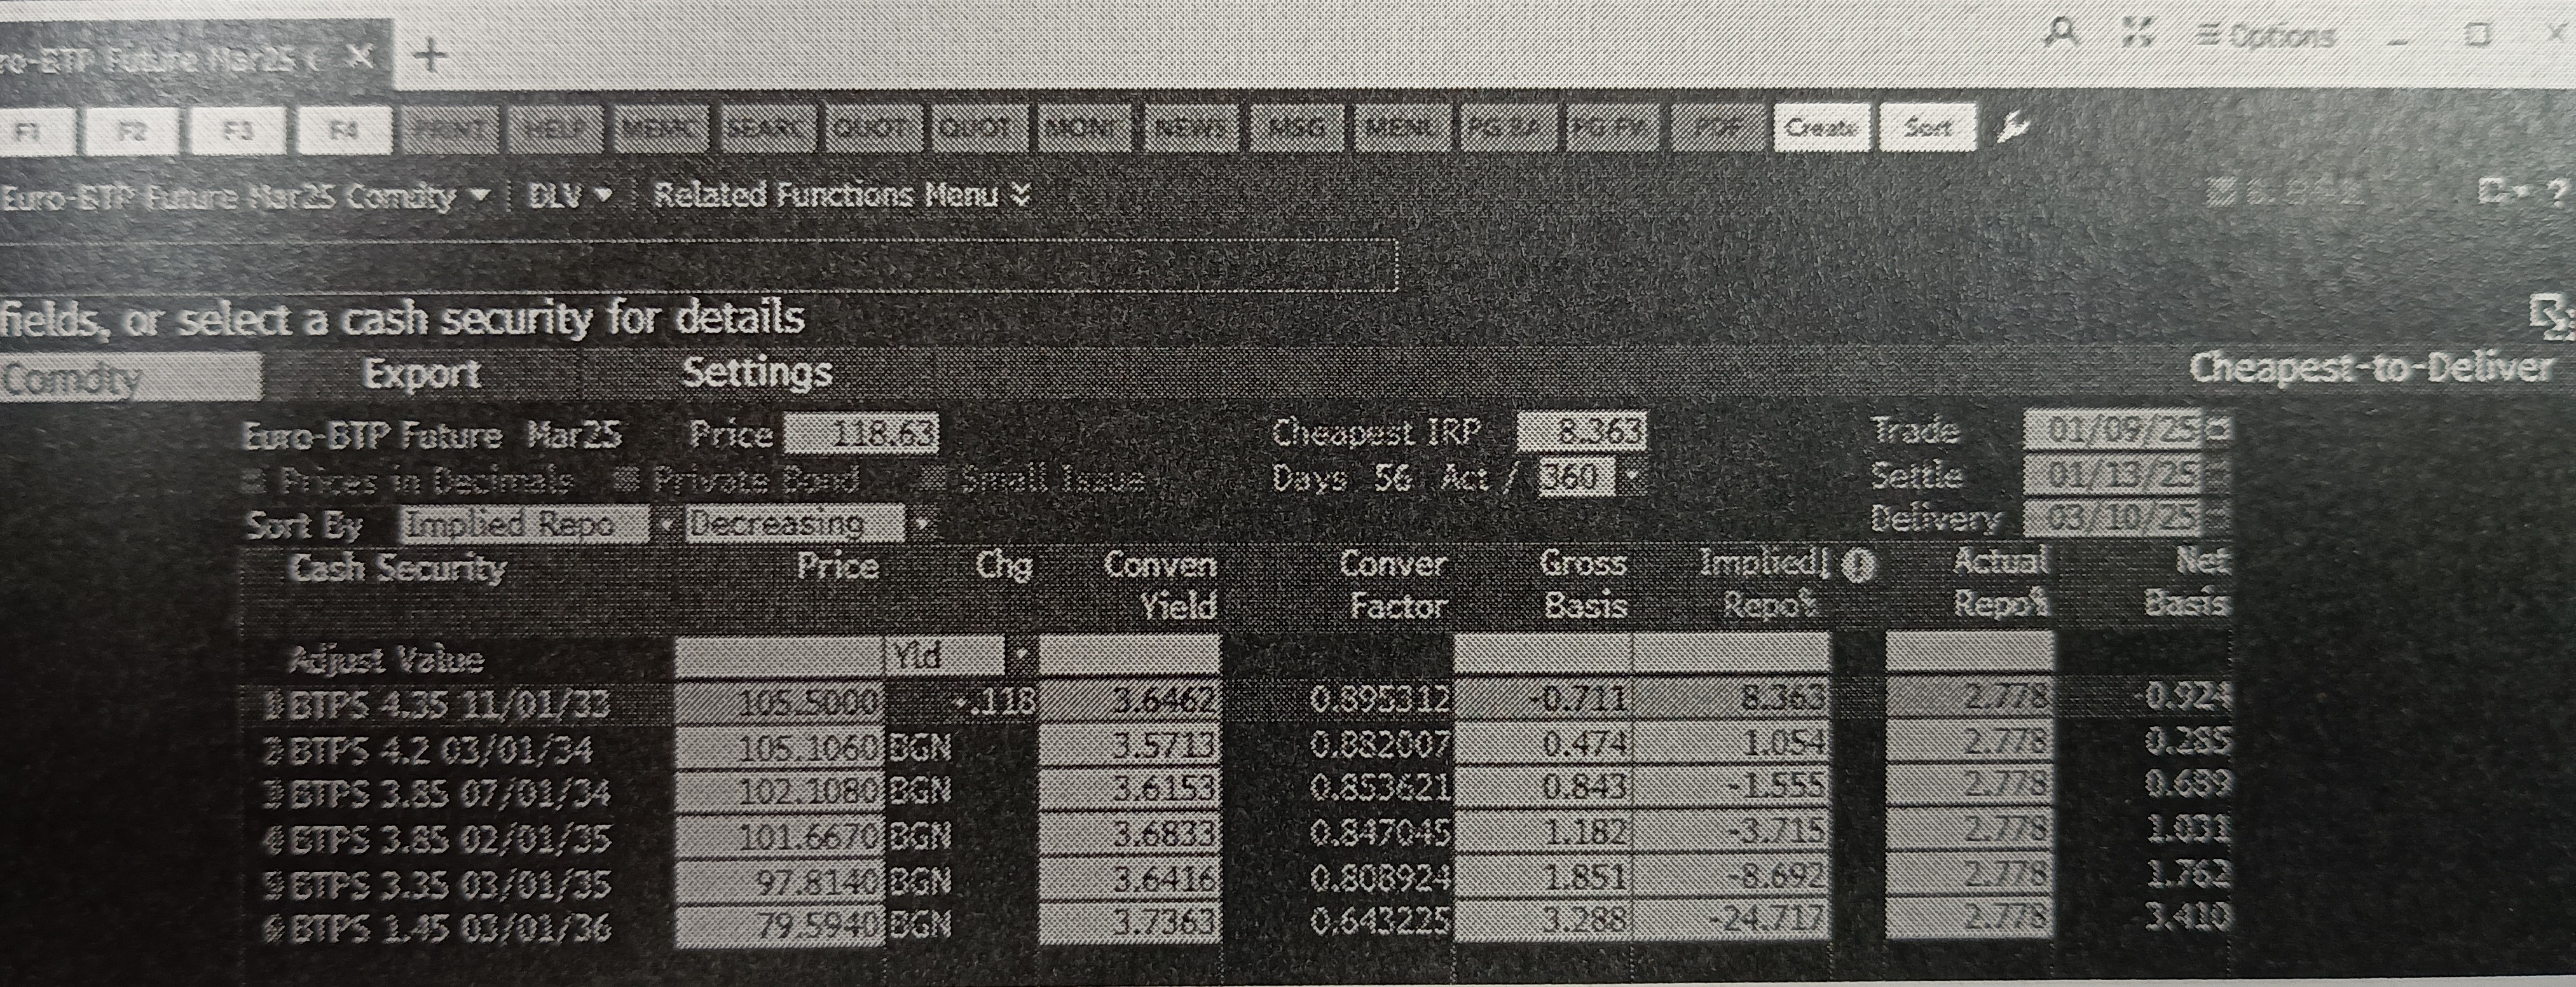
\includegraphics[width=0.9\linewidth]{immagine_compito_27_01_2026}
	\caption{10y nominal rate and 10y inflation swap.}
\end{figure}

\makeemptybox{5cm}
%\fillwithdottedlines{5cm}
\begin{solution}
\end{solution}

%%%%%%%%%%%%%%%%%%%%%%%%%%%%%%%%%%%%%
\question 
Describe the equation for the return attribution model by Brinson, Hood and Beebower (BHB).
\begin{parts}
	\part Explain the difference between Allocation Effect and Security Selection Effect.
	\part Imagine that your portfolio is underweight Tech (10\% vs 20\% Benchmark) and the Tech sector is up 15\%. The Tech stocks in your portfolio are up only 25\%. Determine the allocation effect and the selection effect and the overall portfolio result wrt to sector.
\end{parts}

\makeemptybox{10cm}

\begin{solution}

\end{solution}

%%%%%%%%%%%%%%%%%%%%%%%%%%%%%%%%%%%%%
\question
Consider two \textbf{independent} assets, A and B. Both are "digital" with the following loss profiles $L$ over 1 year horizon:
\begin{itemize}
	\item A: has a 4\% probability of a loss of \$100 million. Otherwise, the loss is \$0;
	\item B: has a 2\% probability of a loss of \$500 million. Otherwise, the loss is \$0.
\end{itemize}

Calculate:
\begin{parts}
	\part 95\% c.l. VaR for each asset A and B separately and for a portfolio $P=A+B$. Check if the additivity property is full-filled;
	\part 95\% c.l. Expected Shortfall (ES) for each asset separately and portfolio $P$. Compare these results with those of part (a).
\end{parts}

%\fillwithdottedlines{5cm}
\makeemptybox{15cm}
\begin{solution}
	\begin{parts}
		\part 95\% c.l. VaR is the 95th quantile of the loss distribution. Hence for both the two assets is \$0 since 95\% of the distribution is in the 0 loss "region" (0.95 < 0.96).
		
		VaR only tells us the "threshold", a risk manager looking only at VaR would see these portfolios as identical in risk.
		
		For portfolio $P$ we have the following loss distribution (the assets are independent):
		\begin{itemize}
			\item \$0 loss: $0.96 \cdot 0.98 \rightarrow 0 \div 0.9408$;
			\item \$100 M loss: $(0.04 \cdot 0.98) \rightarrow 0.9408 \div 0.9800$;
			\item \$500 M loss: $(0.96 \cdot 0.02) \rightarrow 0.9800 \div 0.9992$;
			\item \$600 M loss: $(0.04 \cdot 0.02) \rightarrow 0.9992 \div 1.0000$.
		\end{itemize}
		
		\begin{equation*}
			\text{VaR}_{95\%}(P)=100M \ge \text{VaR}_{95\%}(A) + \text{VaR}_{95\%}(B) = 0M
		\end{equation*}
		
		VaR violates additivity. The risk of losses increases diversifying the portfolio, which is in contrast with basic financial principles.
		
		\part ES is the average loss in the worst $(1-\alpha)\%$ quantile. For the single assets we get
		
		\begin{gather*}
			\text{ES}(A) = \frac{0.04\cdot 100 + 0.01\cdot 0}{0.05} = \$80 M \\
			\text{ES}(B) = \frac{0.02\cdot 500 + 0.03\cdot 0}{0.05} = \$200 M \\	
		\end{gather*}
		
		ES looks at the entire area under the tail. It correctly identifies Portfolio B as significantly riskier because it accounts for the magnitude of the "blow-up" beyond the threshold.
		
		For the portfolio $P$ instead:
		\begin{equation*}
			\text{ES}(P) = \frac{0.0392\cdot 100 + 0.0192\cdot 500 + 0.0008\cdot 600}{0.05} = \$280 M 
		\end{equation*}
		
		Note that ES is mathematically proven to be a Coherent Risk Measure. It always satisfies additivity, ensuring that a diversified portfolio never appears riskier than the sum of its parts.
	\end{parts}
	
\end{solution}

%%%%%%%%%%%%%%%%%%%%%%%%%%%%%%%%%%%%%

\question 
Consider the following market data:
\begin{itemize}
	\item risk free rate ($R_f$): $3\%$
	\item expected return of the market ($E[R_m]$): $10\%$
	\item market variance ($\sigma^2_m$): $0.04$
\end{itemize}

Using the CAPM:
\begin{parts}
	\part compute the expected return of asset A, knowing its $\beta_A = 1.5$.
	\part Consider asset B, which currently has a return of $8,6\%$. From a historical analysis the asset has $\beta_B = 0.9$. Determine if the asset is correctly valued, undervalued or overvalued using Jensen-alpha ($\alpha = R_{B,mkt} - E[R_B]$).
	%\part Decompose asset A total variance ($\sigma^2_A$) among systematic and idiosyncratic knowing that its residual variance is $\sigma^2(\epsilon_A) = 0.05$.
	\part An investor builds a portfolio made of $40\%$ of asset A and $60\%$ in a risk free asset. Compute $\beta_P$ and its expected return.
\end{parts}
\makeemptybox{15cm}

\begin{solution}
	\begin{parts}
		\part Using the Security Market Line (SML) equation:
		\begin{equation*}
			\mathbb{E}[R_A] = R_f + \beta_A (E[R_m] - R_f)
		\end{equation*}
		Replacing the values:
		\begin{equation*}
			\mathbb{E}[R_A] = 0.03 + 1.5 \cdot (0.10 - 0.03) = 0.03 + 0.105 = 13.5\%
		\end{equation*}
		\part To valuate asset B we need to compare its market return ($R_{B,mkt}$) with the theoretical return predicted by the CAPM ($E[R_B]$):
		\begin{equation*}
			\mathbb{E}[R_B] = 0.03 + 0.9 \cdot (0.10 - 0.03) = 0.03 + 0.063 = 9.3\%
		\end{equation*}
		Finally the Jensen-alpha:
		\begin{equation*}
			\alpha_B = R_{B,mkt} - E[R_B] = 8.6\% - 9.3\% = -0.7\%
		\end{equation*}
		Since $\alpha_B < 0$, the asset is \textbf{overvalued}. Its actual return is not enough to remunerate the associated systematic risk ($\beta=0.9$).
		%		\part To decompose the variance in a linear model:
		%		\begin{equation*}
			%			\sigma^2_A = \beta_A^2 \sigma^2_m + \sigma^2(\epsilon_A)
			%		\end{equation*}
		%		\begin{itemize}
			%			\item \textbf{Systematic risk}: $\beta_A^2 \sigma^2_m = (1,5)^2 \times 0,04 = 2,25 \times 0,04 = 0,09$
			%			\item \textbf{Idiosyncratic risk}: $\sigma^2(\epsilon_A) = 0,05$
			%			\item \textbf{Total variance}: $0,09 + 0,05 = 0,14$
			%		\end{itemize}
		\part The portfolio beta is the weighted average of asset betas:
		\begin{equation*}
			\beta_P = w_A \beta_A + w_{rf} \beta_{rf} = 0.4 \times 1.5 + 0.6 \times 0 = 0.6
		\end{equation*}
		The expected return can be computed with the SML using $\beta_P$:
		\begin{equation*}
			E[R_P] = R_f + \beta_P (E[R_m] - R_f) = 0.03 + 0.6 \times (0.10 - 0.03) = 7.2\%
		\end{equation*}
	\end{parts}
\end{solution}

%%%%%%%%%%%%%%%%%%%%%%%%%%%%%%%%%%%%%

\question 
Consider a Payer IRS with a notional $N = €10$M, 3-year maturity and annual payments. The swap fixed rate is $K = 2.0\%$.

Due to macroeconomic tensions, the interest rate term structure steepened:
\begin{itemize}
	\item $L_1$ decreases to $0.50\%$
	\item $L_2$ increases to $2.50\%$
	\item $L_3$ increases al $3.50\%$
\end{itemize}

Assuming constant discount factors to: $DF_1=0.98$, $DF_2=0.96$, $DF_3=0.94$:

\begin{parts}
	\part compute the IRS swap-rate;
	\part determine the swap NPV for the party paying fixed and explain why the NPV is positive even if the short-term rate decreases.
\end{parts}
\makeemptybox{10cm}

\begin{solution}
	\begin{parts}
		\part The swap-rate ($S_{mkt}$) is the weighted average of the forward rates with respect to the discount factors:
		\[ S_{mkt} = \frac{\sum_{i=1}^3 DF_i \cdot L_i}{\sum_{i=1}^3 DF_i} \]
		\[ S_{mkt} = \frac{(0.98 \cdot 0.005) + (0.96 \cdot 0.025) + (0.94 \cdot 0.035)}{0.98 + 0.96 + 0.94} \]
		\[ S_{mkt} = \frac{0.0049 + 0.024 + 0.0329}{2.88} = \frac{0.0618}{2.88} \approx 2.146\% \]
		\part The contract value results
		\[ NPV = N \times (S_{mkt} - K) \times \text{Annuity} \]
		\[ NPV = 10000000 \times (0.02146 - 0.0200) \times 2.88 = €42048 \]
		The NPV is positive because a 3y-swap has a greater duration for longer maturities. 2 and 3 years interest rates increase overcome the decrease at 1 year, globally increasing the swap value.
	\end{parts}
\end{solution}

\end{questions}
\end{document}
